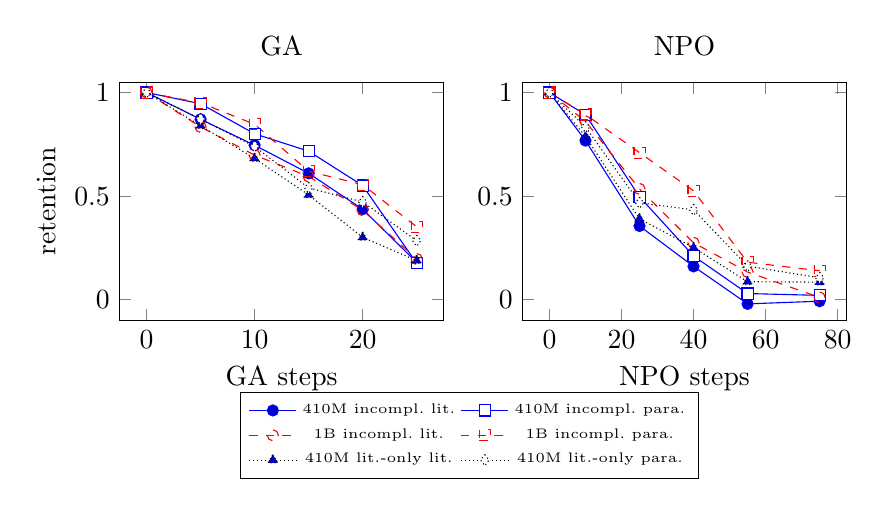
\begin{tikzpicture}
\begin{axis}[name=ga, width=0.47\textwidth, height=0.38\textwidth, xlabel={GA steps},
  ylabel={retention}, ymin=-0.1, ymax=1.05, title={GA}, legend columns=2,
  legend style={font=\tiny, at={(1.08,-0.3)}, anchor=north}]
\addplot+[mark=*, blue] coordinates {(0,1.000) (5,0.871) (10,0.746) (15,0.610) (20,0.437) (25,0.180)};
\addplot+[mark=square*, blue, mark options={fill=white}] coordinates {(0,1.000) (5,0.946) (10,0.801) (15,0.717) (20,0.551) (25,0.176)};
\addplot+[mark=o, red, dashed] coordinates {(0,1.000) (5,0.834) (10,0.698) (15,0.595) (20,0.432) (25,0.197)};
\addplot+[mark=square, red, dashed, mark options={fill=white}] coordinates {(0,1.000) (5,0.950) (10,0.847) (15,0.620) (20,0.555) (25,0.352)};
\addplot+[mark=triangle*, black, densely dotted] coordinates {(0,1.000) (5,0.840) (10,0.682) (15,0.506) (20,0.301) (25,0.189)};
\addplot+[mark=diamond*, black, densely dotted, mark options={fill=white}] coordinates {(0,1.000) (5,0.872) (10,0.740) (15,0.540) (20,0.472) (25,0.285)};
\legend{410M incompl.\ lit., 410M incompl.\ para., 1B incompl.\ lit., 1B incompl.\ para., 410M lit.-only lit., 410M lit.-only para.}
\end{axis}
\begin{axis}[at={(ga.east)}, anchor=west, xshift=1.0cm, width=0.47\textwidth,
  height=0.38\textwidth, xlabel={NPO steps}, ymin=-0.1, ymax=1.05, title={NPO}]
\addplot+[mark=*, blue] coordinates {(0,1.000) (10,0.768) (25,0.356) (40,0.161) (55,-0.020) (75,-0.007)};
\addplot+[mark=square*, blue, mark options={fill=white}] coordinates {(0,1.000) (10,0.893) (25,0.497) (40,0.211) (55,0.030) (75,0.021)};
\addplot+[mark=o, red, dashed] coordinates {(0,1.000) (10,0.861) (25,0.535) (40,0.275) (55,0.134) (75,0.011)};
\addplot+[mark=square, red, dashed, mark options={fill=white}] coordinates {(0,1.000) (10,0.894) (25,0.710) (40,0.526) (55,0.181) (75,0.140)};
\addplot+[mark=triangle*, black, densely dotted] coordinates {(0,1.000) (10,0.788) (25,0.390) (40,0.252) (55,0.087) (75,0.085)};
\addplot+[mark=diamond*, black, densely dotted, mark options={fill=white}] coordinates {(0,1.000) (10,0.834) (25,0.468) (40,0.434) (55,0.162) (75,0.106)};
\end{axis}
\end{tikzpicture}
